\chapter{Characterization of sharing-behavior of STM applications}\label{chap:charact}

For a successful thread mapping, it is necessary to perform an in-depth analysis of STM applications, for instance, if the memory access pattern changes in each execution; the number of addresses accessed inside transactions, etc. This analysis is important to guide decisions regarding mapping, such as determining if an application is suitable for a thread mapping based on communication behavior and defining the type of mapping policy (static or dynamic). %In the context of this paper, communication and sharing are used interchangeably and have the same meaning.

In this chapter, we characterize the applications from \texttt{STAMP}~\cite{STAMP}, by gathering sharing information through the proposed mechanism in Chapter~\ref{chap:mechanism}, providing information to guide thread placement based on their sharing behavior. The \texttt{STAMP} benchmark was developed with the intention to represent realistic workload characteristics and different application domains. Besides, \texttt{STAMP} covers a wide range of transactional behavior, for instance, varying transaction lengths, contention, quantity of transactions, etc. Hence, we expect that the characterization done in this chapter could represent a wide range of real STM applications. Using the proposed mechanism we are able to gather information about the suitability for thread mapping of each application, its communication pattern, and its dynamic behavior, among others. We also show how this mechanism can be used to detect false sharing of cache lines of STM operations.


\section{Methodology of the Characterization}\label{sec:methodology}
%This section discusses the methodology of the characterization.

\subsection{Detecting sharing in STM applications}
The characteristics of memory access behavior presented in this thesis are based on the communication matrices of applications. To extract the matrices we have used the mechanism proposed in Chapter~\ref{chap:mechanism}. %This mechanism is triggered on each transactional data access operation (read or write). When at least two different threads accessed the same memory address, a communication event between them is stored in a communication matrix. Examples of communication matrices are shown in Fig.~\ref{fig:FirstQMatrices}. Axes show threads IDs. The mechanism was implemented in the \texttt{TinySTM} library~\cite{TinySTM2}, version 1.0.5. \texttt{TinySTM} was configured to use the default configuration: \emph{lazy} version management, \emph{eager} conflict detection and contention manager \emph{suicide}.
%
\texttt{STAMP} was compiled with gcc~8.3.0. If not specified otherwise, all applications were executed ten times using 64 threads and the default input parameters shown in \tablename~\ref{tab:defaultParams}. We also used the same Xeon machine described on Section~\ref{sec:mechMethodology} to run the experiments.
 %, where \thNumber~represents the number of threads. 
%Most parameters are larger than the largest ones suggested in the original paper~\cite{STAMP} to achieve more substantial execution times on modern machines. %\new{The idea to change it was to make each application run for at least ten seconds.}

%\begin{table}[!tb]
%	\small
%	\centering
%	\caption{Default arguments for the programs used in the experiments.}
%	\label{tab:defaultParams}
%	\begin{tabular}{@{}ll@{}}
%		\toprule
%		Application & Arguments                                          \\ \midrule
%		bayes                & \texttt{-v32 -r8192 -n10 -p40 -i2 -e8 -s1 -t \thNumber}                \\
%		genome               & \texttt{-g49152 -s256 -n33554432 -t \thNumber}                         \\
%		intruder             & \texttt{-a10 -l128 -n262144 -s1 -t \thNumber}                          \\
%		kmeans               & \texttt{-m40 -n40 -t0.00001 -i random-n65536-d32-c16.txt -p \thNumber}\\
%		labyrinth            & \texttt{-i random-x1024-y1024-z9-n1024.txt -t \thNumber}               \\
%		ssca2                & \texttt{-s21 -i1.0 -u1.0 -l3 -p3 -t \thNumber}                         \\
%		vacation             & \texttt{-n4 -q90 -u100 -r1310720 -t16777216 -c \thNumber}              \\
%		yada                 & \texttt{-a15 -i ttimeu1000000.2 -t \thNumber}                          \\
%		\bottomrule
%	\end{tabular}
%\end{table}
%\subsection{Machine}

%Applications were executed on an eight-socket Intel Xeon E5-4650 system, running Linux kernel 4.19.0-9. Each socket has 12 2-HT cores, totaling 96 cores. Each socket corresponds to a NUMA node (for a total of 8 NUMA nodes), and 12$\times$ 32 KB L1d, 12$\times$ 32 KB L1i, 12$\times$ 256 KB L2 and 30 MB L3 caches.

\subsection{Mean squared error (MSE)}\label{sec:MSE}

Since the analysis of the communication behavior of the applications is based on communication matrices, we used \emph{Mean squared error} (MSE)~\cite{MSE} metric to compare the difference between them, which has been used in prior work for this purpose~\cite{Diener:2016:2}. The equation to calculate the MSE is shown in Eq.~\ref{eq:MSE}.

\begin{samepage}
	\begin{equation}
		MSE(A, B) =  \frac{1}{N^2}\sum_{i=0}^{N-1}\sum_{j=0}^{N-1}(A[i,j]-B[i,j])^2
		\label{eq:MSE}
	\end{equation}
	where:
	\begin{conditions}
		A, B     &  input matrices \\
		N        &  matrix order, i.e., number of threads \\
		i,j      &  matrix indexes
	\end{conditions}
\end{samepage}

If the MSE of two matrices is zero, then the matrices are exactly the same. Higher MSE values indicate higher differences. This metric is useful to compare, for instance, if the memory access behavior of one application changes on each execution. %In that case, values closer to zero indicate that the matrices are more similar.

\subsection{Experiments}\label{sec:experiments}

We performed the following experiments to characterize the sharing behavior of the \texttt{STAMP} applications:

\begin{enumerate}
	\item We collected information about the total of accessed addresses inside the STM library. The information is useful to understand how much data is accessed by STM operations (Section~\ref{sec:falseSharing}).
	
	\item We executed the same application ten times to verify if the communication pattern changes between executions. This experiment will show if a communication matrix collected in a previous execution can be used to make a static thread mapping (Section~\ref{sec:sameDIffExecs}).
	
	\item We executed the same application ten times, changing the input parameters from the default. This experiment will show if it is possible to use a collected communication matrix with different input parameters to make a static thread mapping (Section~\ref{sec:newInput}).
	
	\item We executed the same application ten times, changing the total number of threads from the previous experiments, with the same goal as in the previous item (Section~\ref{sec:differentThreads}).
	
	\item We collected the communication matrix several times during the execution of an application, to determine if an application needs an online mechanism to detect the sharing behavior and perform the thread mapping multiple times during execution (Section~\ref{sec:dynamicBehavior}).
\end{enumerate}

\section{Characterization of sharing behavior}\label{sec:charact}

This section presents the characterization of the \texttt{STAMP} applications, regarding memory access behavior.

\subsection{STM memory access information}\label{sec:falseSharing}

The first data set is not directly related to sharing behavior but is useful to explain further the behavior of applications.
The total number of distinct memory addresses accessed by STM operations was collected as well as the total number of accesses made to these addresses such as read or write operations. With this data, it is possible to calculate other information:
\begin{itemize}
	\item \textbf{Number of distinct cache lines}: This was calculated based on the default cache line of most current microarchitectures, 64 bytes.
	
	\item \textbf{Number of distinct pages}: This was calculated based on the default page size of many current microarchitectures, 4096 bytes.
	
	\item \textbf{Percentage of cache lines with false sharing}: We consider that a cache line has false sharing when multiple threads perform STM operations on more than one word at the same line.
\end{itemize}

\begin{table}[ht]
	\centering
	\caption{Analysis of accessed STM memory addresses in STAMP applications.}
	\label{tab:falseSharing}
\begin{tabular}{l@{\hspace*{10pt}}r@{\hspace*{10pt}}r@{\hspace*{10pt}}r@{\hspace*{10pt}}r@{\hspace*{10pt}}r}
	\toprule
	{Application} & \multicolumn{1}{c}{{\begin{tabular}[c]{r}Distinct \\ addresses\end{tabular}}} & \multicolumn{1}{c}{{\begin{tabular}[c]{@{}r@{}}Distinct \\ cache lines\end{tabular}}} & \multicolumn{1}{c}{{\begin{tabular}[c]{@{}r@{}}Distinct \\ pages\end{tabular}}} & \multicolumn{1}{c}{{\begin{tabular}[c]{@{}r@{}}Total \\ accesses\end{tabular}}} & \multicolumn{1}{c}{{\begin{tabular}[c]{@{}r@{}}\% of lines with  \\ false  sharing\end{tabular}}} \\ \midrule
	bayes                & 1,082                                                                                      & 497                                                                                         & 122                                                                                     & 15,928,303                                                                             & 89.33                                                                                    \\
	kmeans               & 682                                                                                        & 101                                                                                         & 4                                                                                      & 833,954,131                                                                            & 100.00                                                                                   \\
	labyrinth            & 824,126                                                                                    & 290,083                                                                                     & 18,213                                                                                 & 1,994,315                                                                              & 83.05                                                                                    \\
	genome               & 19,750,104                                                                                 & 11,216,870                                                                                  & 452,651                                                                                & 2,840,508,725                                                                          & 36.21                                                                                    \\
	intruder             & 23,292,164                                                                                 & 8,131,906                                                                                   & 297,629                                                                                & 4,105,619,590                                                                          & 99.00                                                                                    \\
	yada                 & 25,055,077                                                                                 & 13,932,226                                                                                  & 848,045                                                                                & 610,446,722                                                                            & 81.38                                                                                    \\
	vacation             & 33,671,744                                                                                 & 10,796,118                                                                                  & 799,129                                                                                & 7,212,365,036                                                                          & 99.08                                                                                    \\
	ssca2                & 91,335,091                                                                                 & 13,907,852                                                                                  & 528,387                                                                                & 270,369,505                                                                            & 99.90                                                                                    \\ \bottomrule
\end{tabular}
\end{table}

Results are shown in \tablename~\ref{tab:falseSharing} and indicate that the applications have different characteristics regarding the number of accessed addresses. \textit{kmeans} has the lowest amount of distinct addresses accessed. However, it has a large number of total accesses made to these addresses. On the other hand, \textit{ssca2} has the largest amount of distinct addresses accessed, but not the largest total of accesses, which belongs to \textit{vacation}.
%
Regarding false sharing, the majority of applications have a large percentage of false sharing. For instance, in \textit{kmeans}, all addresses share common cache lines. On the other hand, \textit{genome} has the least amount of false sharing which indicates that more than half of the accessed addresses has at least 64 bytes or the addresses that conflict in the same cache line are accessed outside the STM library.

\subsection{Stability of sharing behavior across different executions}\label{sec:sameDIffExecs}

The goal of this experiment is to determine if the communication pattern changes across different executions of the same application, using the same input parameters and number of threads. To answer this question, we executed all applications one time and collected the communication matrix, to be used as a baseline for comparison. After that, we run each application nine more times, collecting the communication matrix in each execution. Then, we calculated the MSE of each resulting matrix, comparing it to the first execution. Results are shown in~\figurename~\ref{fig:averageFirstQ}.

\begin{figure}[!t]
	\centering
	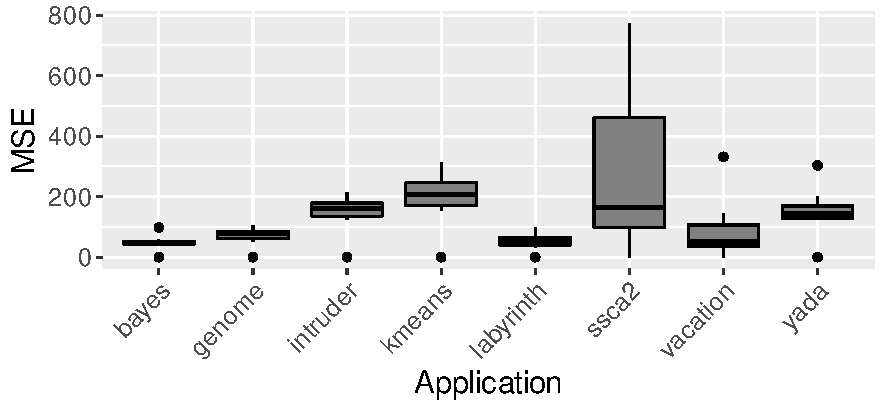
\includegraphics[width=\fullImageWidth\textwidth]{figures/sharingBehavior/FirstQ/0.graph.pdf}
	\caption{Stability of the sharing behavior across different executions.}
	\label{fig:averageFirstQ}
\end{figure}

Some applications, for instance \emph{bayes}, \emph{genome} and \emph{labyrinth}, present the same communication behavior in all executions. This observation can be visualized in two different communication matrices of \emph{bayes} (\figurename~\ref{fig:FirstQBayes1} and \figurename~\ref{fig:FirstQBayes2}). Axes show threads IDs.
\begin{figure}[!t]
	\centering
	\subfigure[bayes]{
		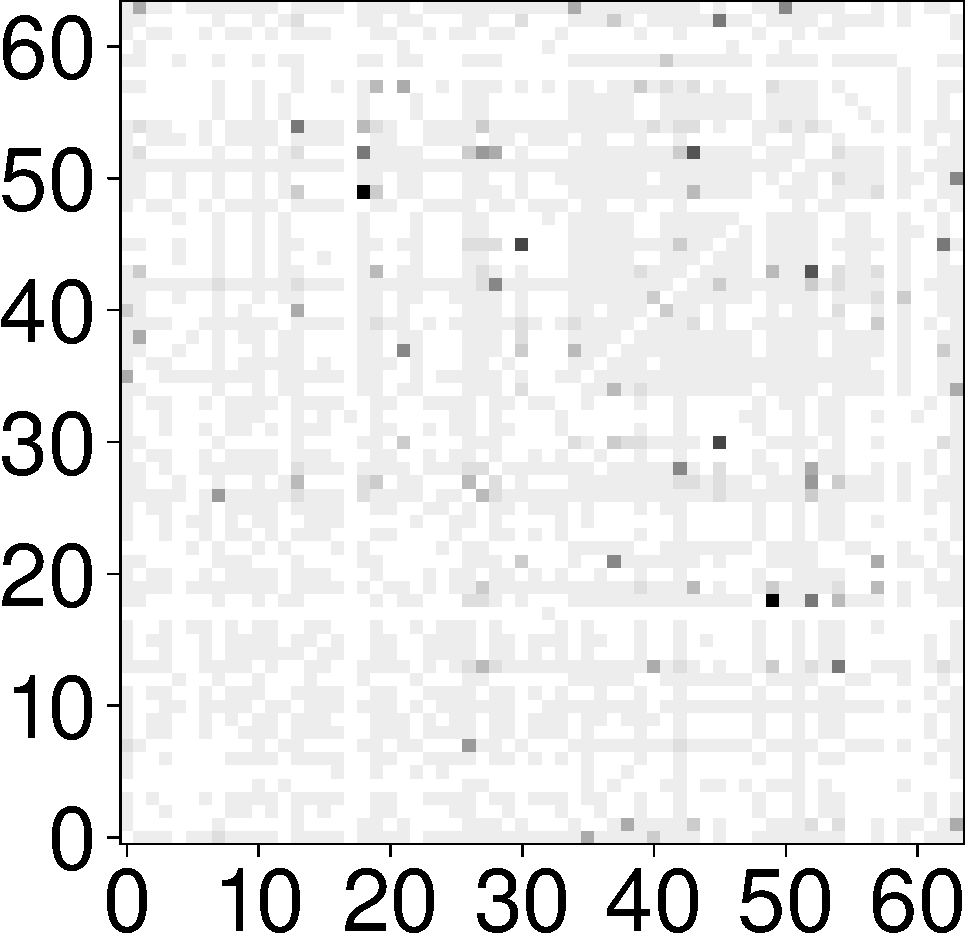
\includegraphics[width=\oneQPage\textwidth]{figures/sharingBehavior/FirstQ/bayes_64.pdf}
		\label{fig:FirstQBayes1}
	}
	\subfigure[bayes]{
		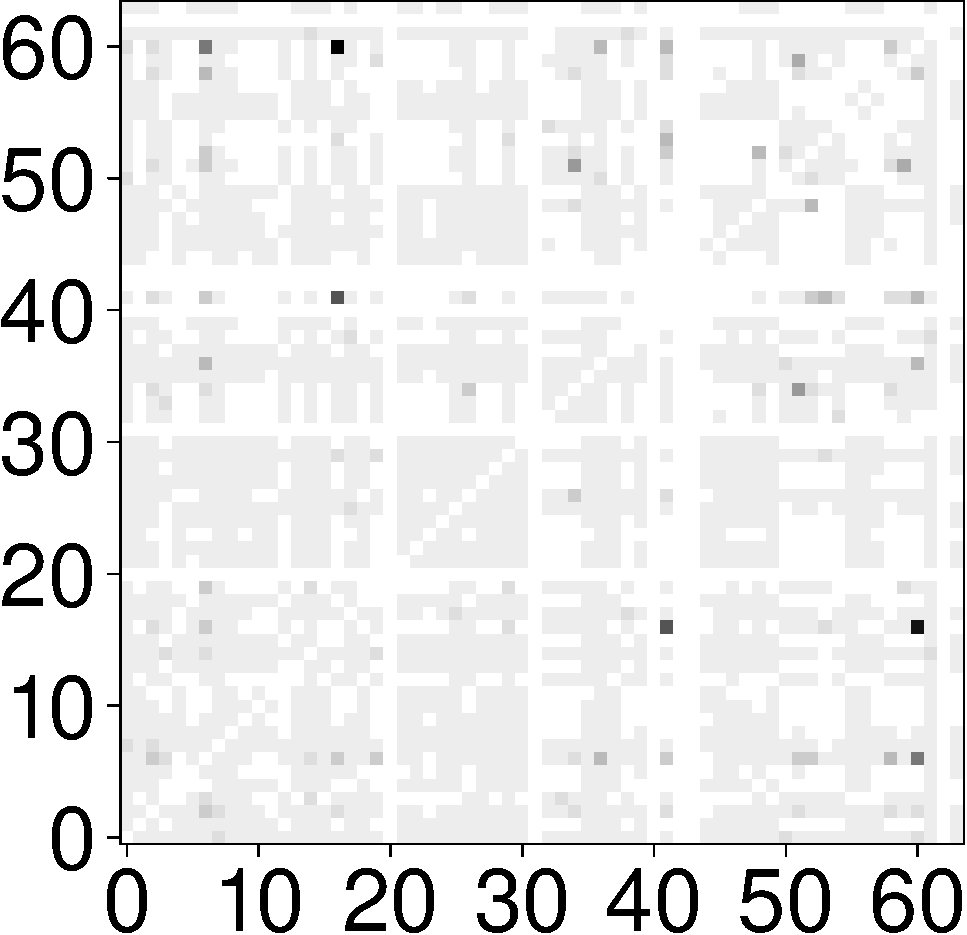
\includegraphics[width=\oneQPage\textwidth]{figures/sharingBehavior/FirstQ/bayes_64_5.pdf}
		\label{fig:FirstQBayes2}
	}
	\subfigure[ssca2]{
		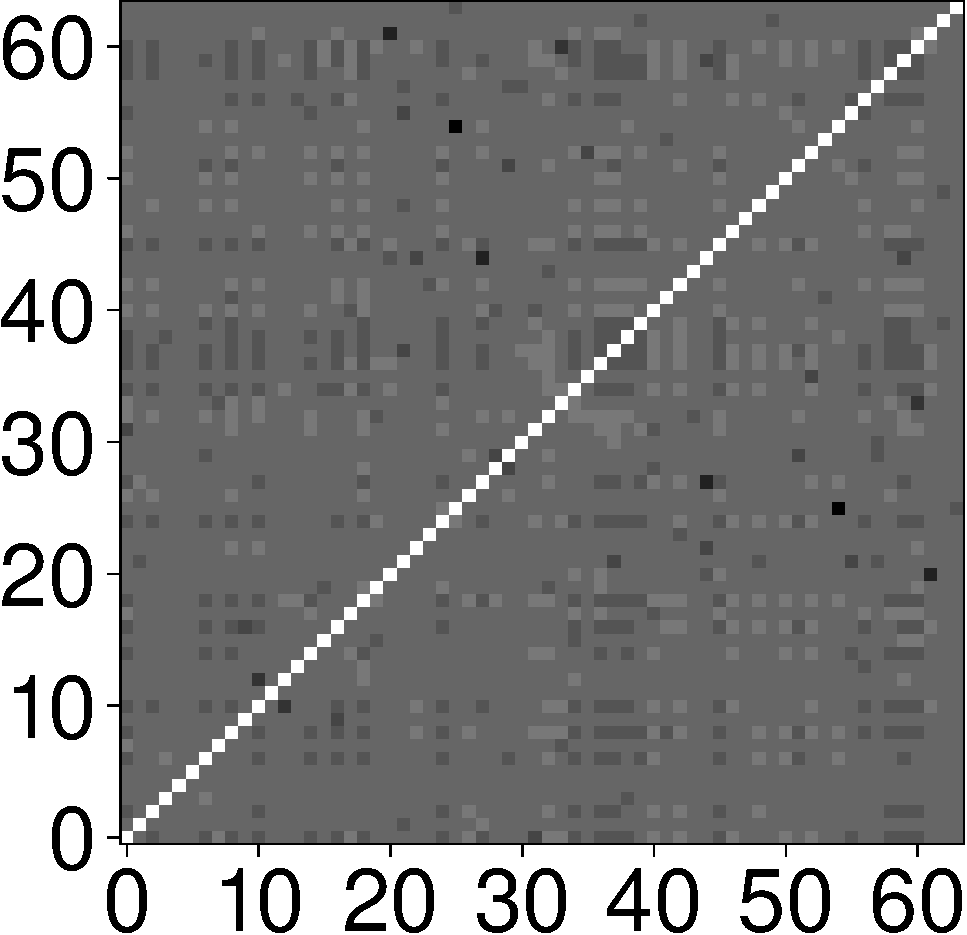
\includegraphics[width=\oneQPage\textwidth]{figures/sharingBehavior/FirstQ/ssca2_64.pdf}
		\label{fig:FirstQssca21}
	}
	\subfigure[ssca2]{
		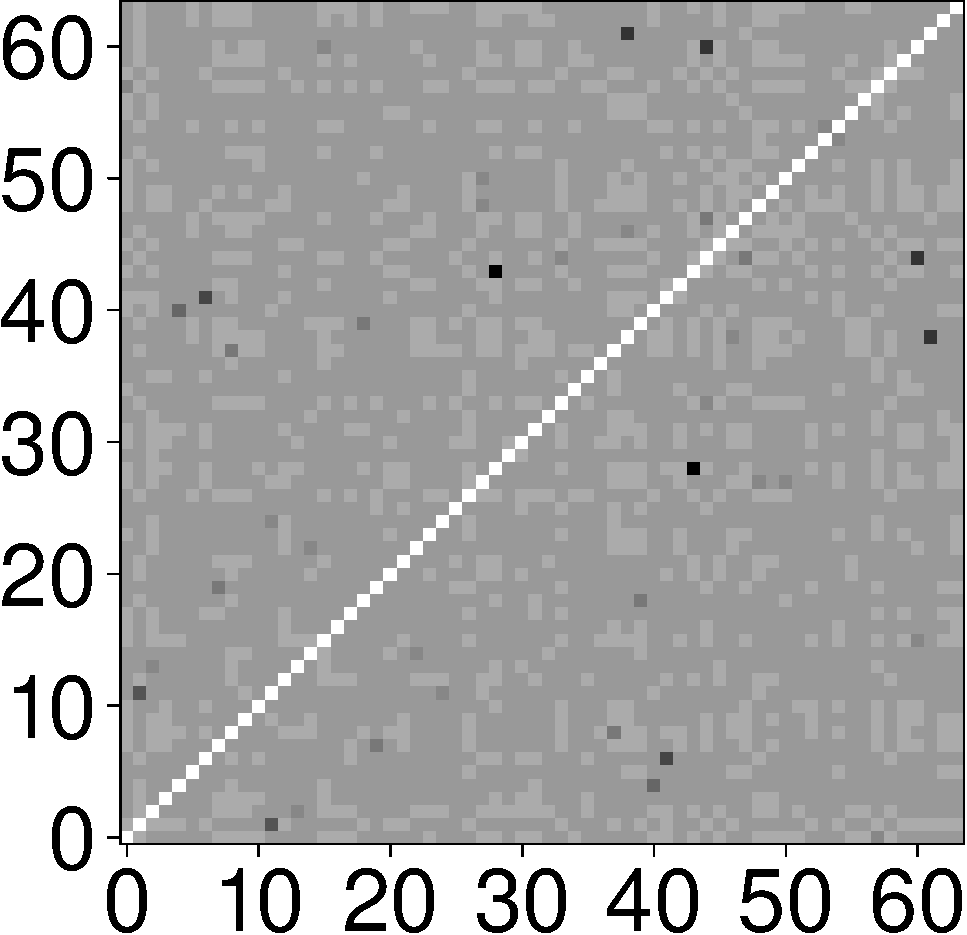
\includegraphics[width=\oneQPage\textwidth]{figures/sharingBehavior/FirstQ/ssca2_64_7.pdf}
		\label{fig:FirstQssca22}
	}
	\caption{Matrices with highest and lowest MSEs between different executions.}
	\label{fig:FirstQMatrices}
\end{figure}
In contrast to \emph{bayes}, \emph{ssca2} presents a not so similar behavior on each execution. However, looking at two \emph{ssca2} matrices (\figurename~\ref{fig:FirstQssca21}) and \figurename~\ref{fig:FirstQssca22}) it is possible to note that although the basic communication behavior is the same (all-to-all \cite{Williams:2009}), the total amount of communication between threads is very different. This can be explained by  the non-deterministic behavior of TM applications, mainly due to the fact that the total number of aborts varies in each execution. More aborts imply in more work to be done, consequently more communication between threads. In that case, even having a higher MSE between executions, \emph{ssca2} has a similar behavior of communication between threads (all-to-all pattern) in all executions.

\subsection{Stability of sharing behavior when changing input parameters}\label{sec:newInput}

For this experiment, instead of using the default input parameters shown in \tablename~\ref{tab:defaultParams}, we used a smaller input data set. The changed parameters are shown in \tablename~\ref{tab:changedParams}.
\begin{table}[!ht]
	\centering
	\caption{Small input parameters used in the experiments in Section~\ref{sec:newInput}.}
	\label{tab:changedParams}
	\begin{tabularx}{\textwidth}{@{}lXl@{}}
	\toprule
	Application & Arguments                                          \\ \midrule
	bayes                & \texttt{-v16 -r4096 -n15 -p40 -i2 -e8 -s1 -t \thNumber}                \\
	genome               & \texttt{-g16384 -s64 -n16777216 -t \thNumber}                         \\
	intruder             & \texttt{-a10 -l64 -n131072 -s1 -t \thNumber}                          \\
	kmeans               & \texttt{-m15 -n15 -t0.00001 -i random-n65536-d32-c16.txt -p \thNumber}\\
	labyrinth            & \texttt{-i random-x512-y512-z7-n512.txt -t \thNumber}               \\
	ssca2                & \texttt{-s18 -i1.0 -u1.0 -l3 -p3 -t \thNumber}                         \\
	vacation             & \texttt{-n4 -q60 -u90 -r1048576 -t4194304 -c \thNumber}              \\
	yada                 & \texttt{-a20 -i ttimeu100000.2 -t \thNumber}                          \\
	\bottomrule
\end{tabularx}
\end{table}
Then, we collected ten communication matrices using the same methodology of Section~\ref{sec:sameDIffExecs}. Lastly, a comparison of the MSE using the default parameters (Section~\ref{sec:sameDIffExecs}) was made, comparing with the small parameters (\tablename~\ref{tab:changedParams}). This comparison is shown in \figurename~\ref{fig:averageSecondQ}.

\begin{figure}[!tb]
	\centering
	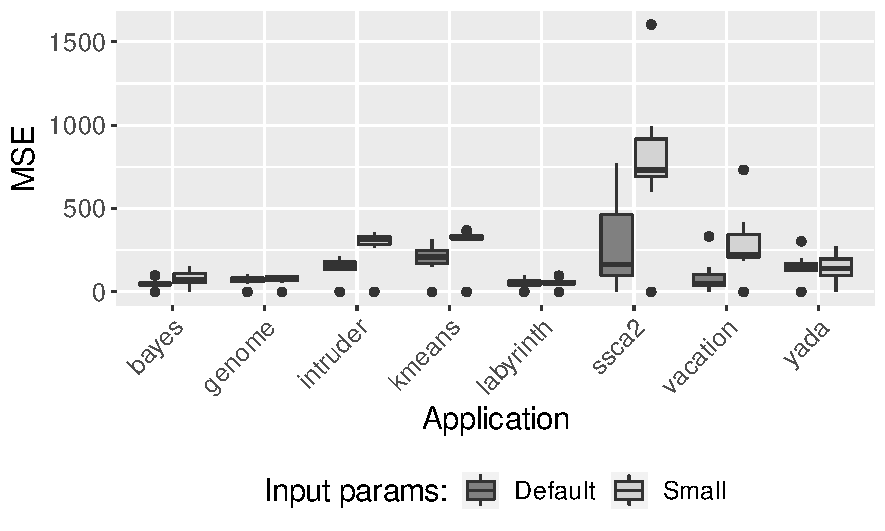
\includegraphics[width=\fullImageWidth\textwidth]{figures/sharingBehavior/SecondQ/0.graph.pdf}
	\caption{Stability of the sharing behavior when changing input parameters.}
	\label{fig:averageSecondQ}
\end{figure}

As in the previous experiment, \emph{ssca2} has a different pattern on each execution. For instance, \figurename~\ref{fig:SecondQssca21} and
\figurename~\ref{fig:SecondQssca22} show two different executions of  \emph{ssca2}, using the small parameters (\tablename~\ref{tab:changedParams}).
\begin{figure}[!tb]
	\centering
	\subfigure[genome-default]{
		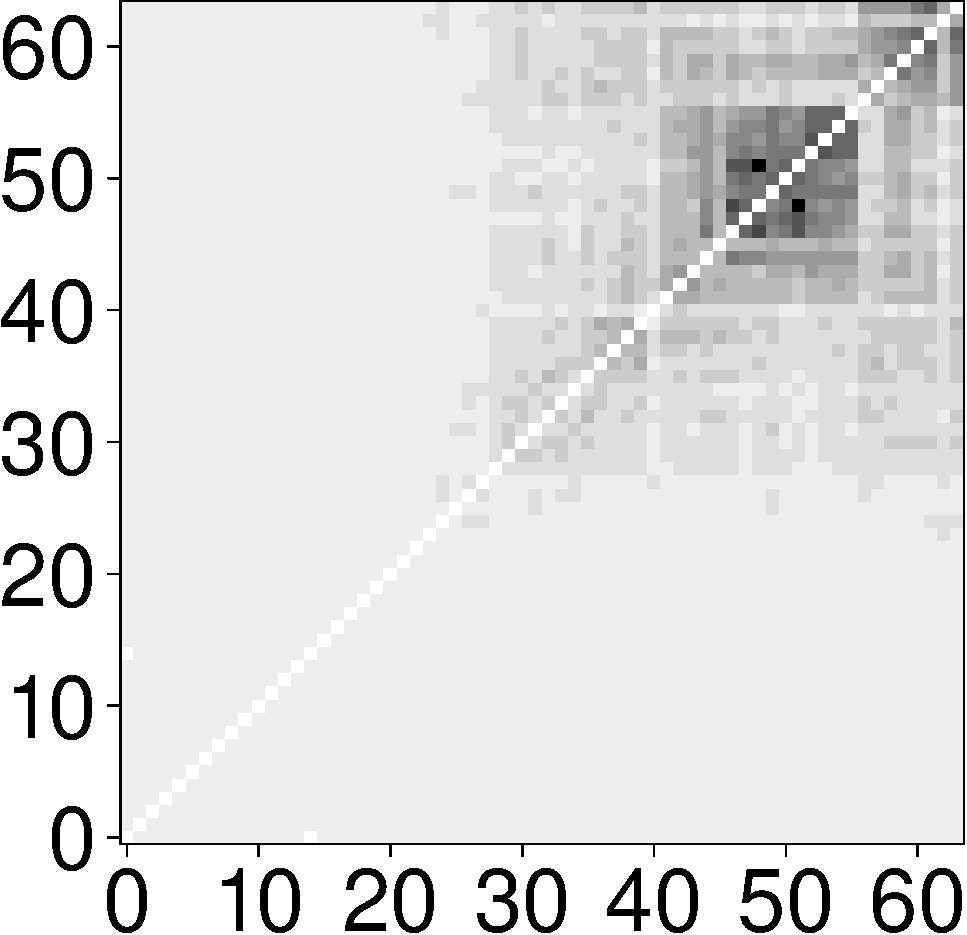
\includegraphics[width=\oneQPage\textwidth]{figures/sharingBehavior/SecondQ/genome_64_2-Default.pdf}
		\label{fig:SecondQgenomeD}
	}
	\subfigure[genome-small]{
		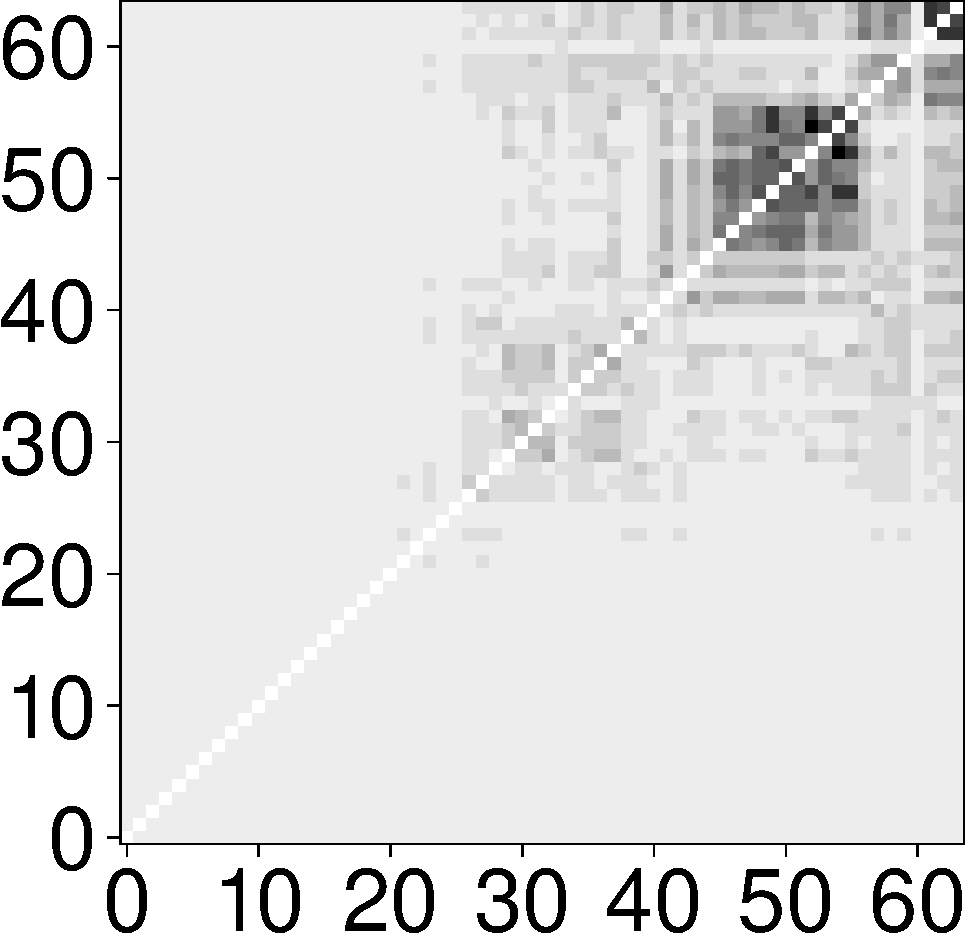
\includegraphics[width=\oneQPage\textwidth]{figures/sharingBehavior/SecondQ/genome_64_3-Changed.pdf}
		\label{fig:SecondQgenomeC}
	}
	\subfigure[ssca2-small]{
		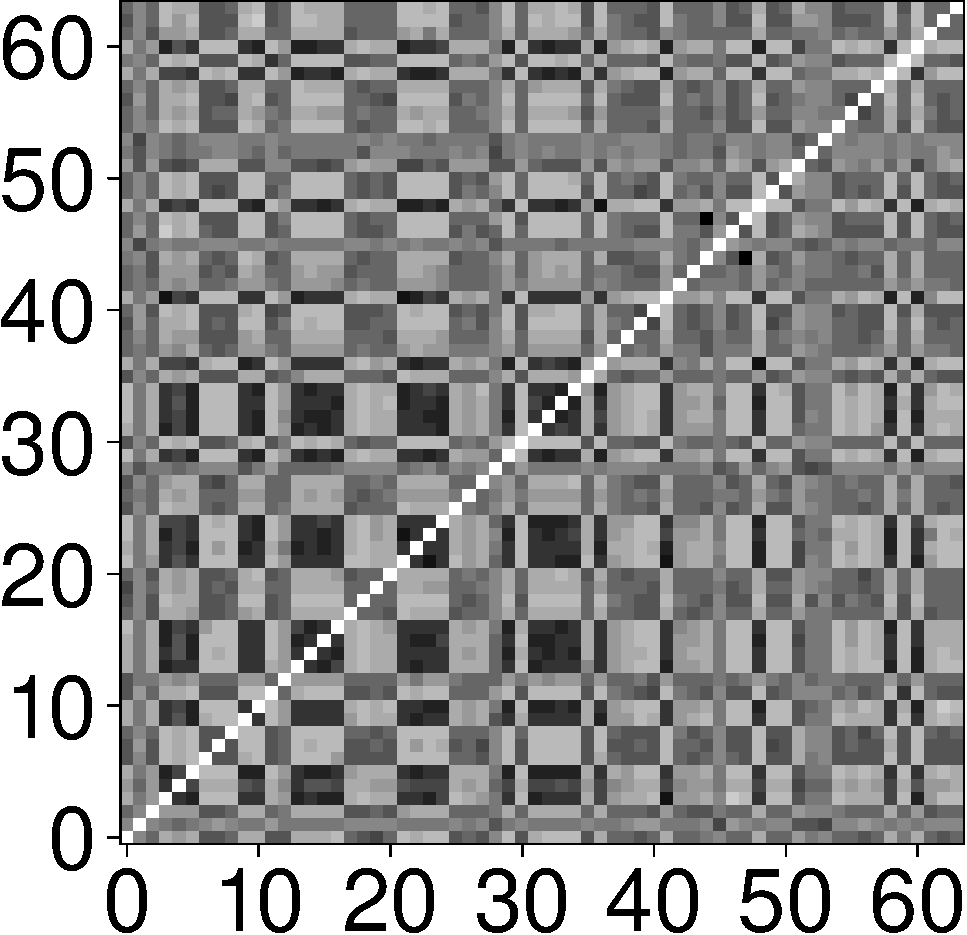
\includegraphics[width=\oneQPage\textwidth]{figures/sharingBehavior/SecondQ/ssca2_64.pdf}
		\label{fig:SecondQssca21}
	}
	\subfigure[ssca2-small]{
		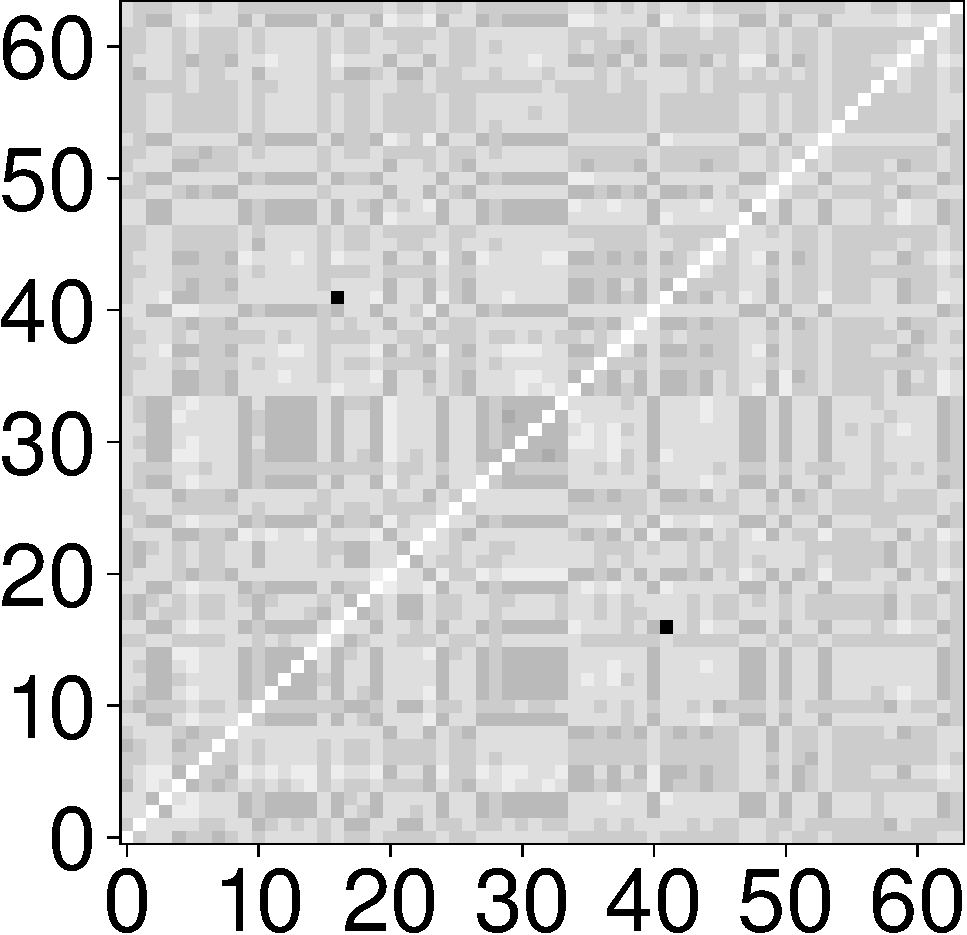
\includegraphics[width=\oneQPage\textwidth]{figures/sharingBehavior/SecondQ/ssca2_64_8.pdf}
		\label{fig:SecondQssca22}
	}
	\caption{Matrices with highest and lowest MSEs.}
	\label{fig:SecondQMatrices}
\end{figure}
However, with the new parameters, it is possible to observe that some groups of threads communicate more often than others (\figurename~\ref{fig:SecondQssca21}). Besides, there is a difference between communication patterns taking into consideration the default and small parameter sets. This can be visualized by comparing \figurename~\ref{fig:FirstQssca21} and \figurename~\ref{fig:SecondQssca21}. Other applications such as \emph{intruder}, \emph{kmeans}, and \emph{vacation} have a small difference between communication patterns when changing input parameters. While others, such as \emph{genome} have almost the same communication pattern, even when changing the input parameters (\figurename~\ref{fig:SecondQgenomeD} and \figurename~\ref{fig:SecondQgenomeC}).

\subsection{Stability of sharing behavior with different numbers of threads}\label{sec:differentThreads}

\figurename~\ref{fig:averageFirstQ} in Section~\ref{sec:sameDIffExecs} showed the communication matrices for 64 threads. We used the same methodology to collect them for 32 and 96 threads, and show the results in \figurename~\ref{fig:averageThirdQ}.
%
\begin{figure}[!t]
	\centering
	\subfigure[32 threads.]{
		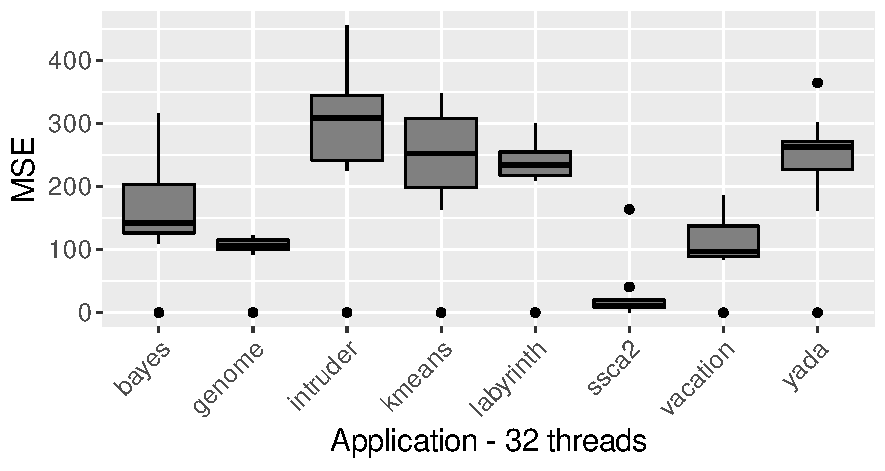
\includegraphics[width=\halfPage\textwidth]{figures/sharingBehavior/ThirdQ/Default32Threads.pdf}
		\label{fig:ThirdQ32Threads}
	}
	\subfigure[96 threads.]{
		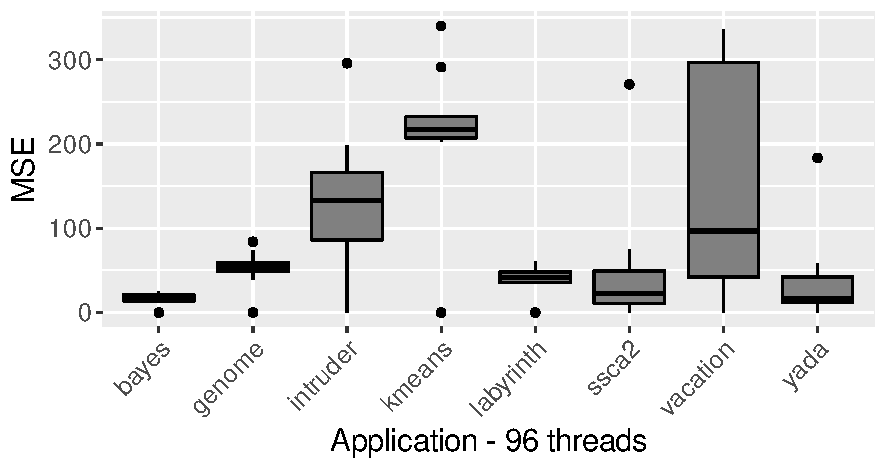
\includegraphics[width=\halfPage\textwidth]{figures/sharingBehavior/ThirdQ/Default96Threads.pdf}
		\label{fig:ThirdQ96Threads}
	}
	\caption{Stability of the sharing behavior when changing the number of threads.}
	\label{fig:averageThirdQ}
\end{figure}
%
The most different behavior occurs with \emph{vacation} and 96 threads. However, looking at the communication pattern of two executions with the highest MSE (\figurename~\ref{fig:ThirdQvacation961} and \figurename~\ref{fig:ThirdQvacation962}) we saw the same behavior for \emph{ssca2} in Section~\ref{sec:sameDIffExecs}.
\begin{figure}[!ht]
	\centering
	\subfigure[genome (32 thr)]{
		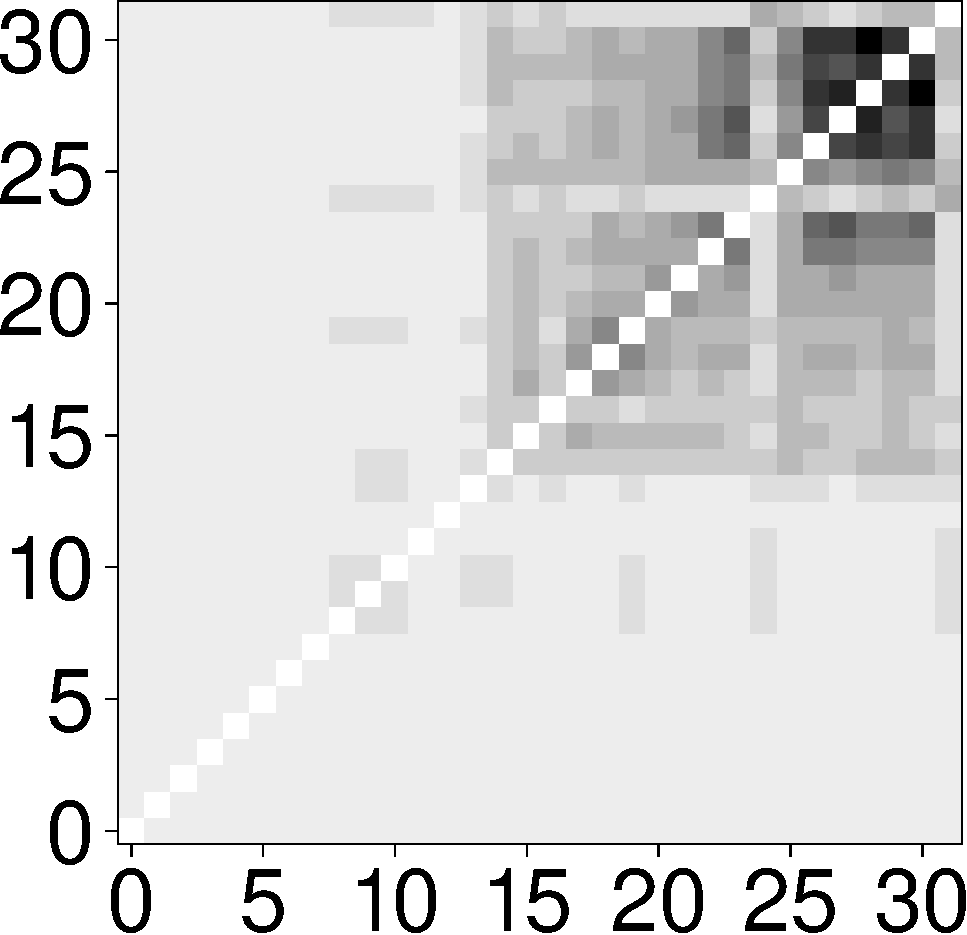
\includegraphics[width=\oneQPage\textwidth]{figures/sharingBehavior/ThirdQ/genome_32.pdf}
		\label{fig:ThirdQgenome321}
	}
	\subfigure[genome (32 thr)]{
		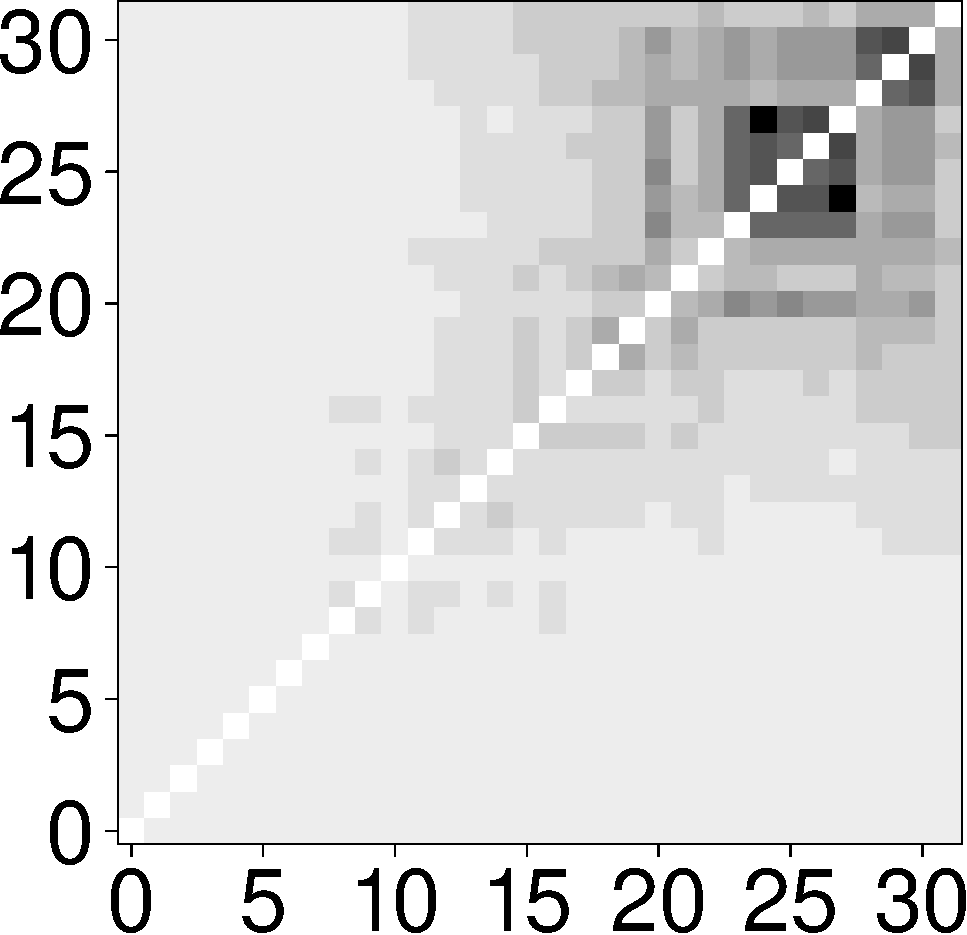
\includegraphics[width=\oneQPage\textwidth]{figures/sharingBehavior/ThirdQ/genome_32_1.pdf}
		\label{fig:ThirdQgenome322}
	}
	\subfigure[vacation (96 thr)]{
		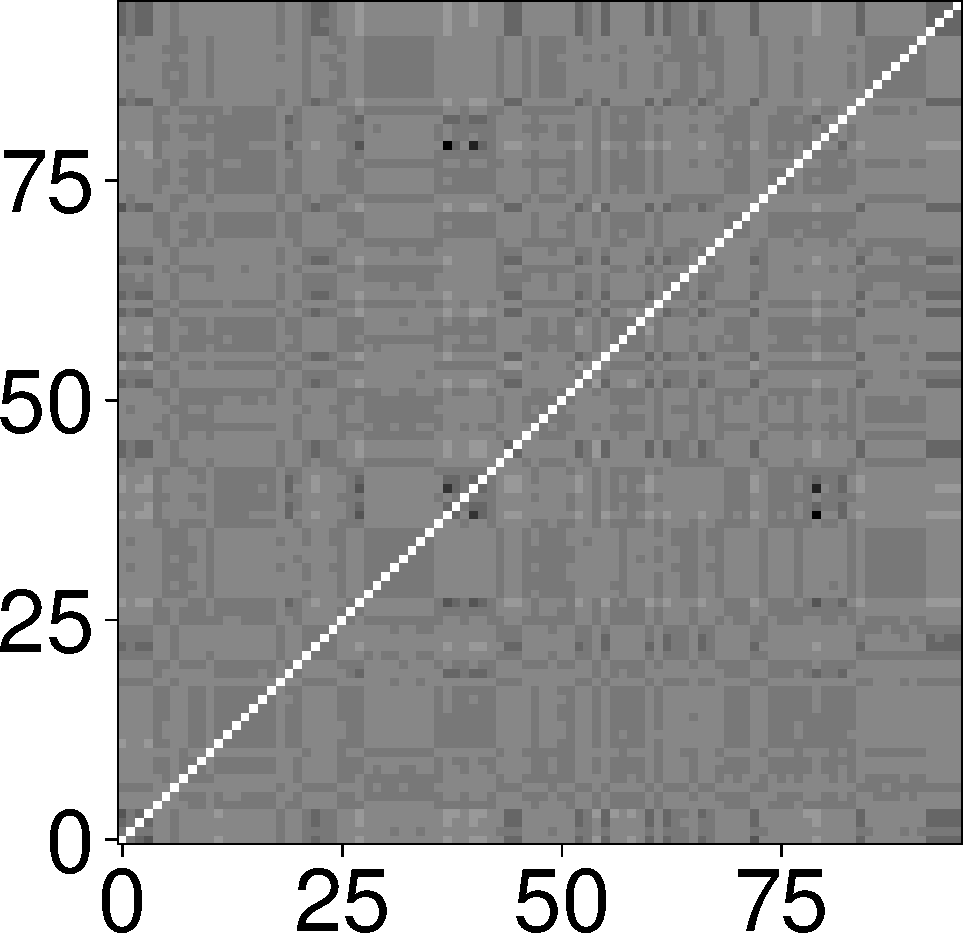
\includegraphics[width=\oneQPage\textwidth]{figures/sharingBehavior/ThirdQ/vacation_96.pdf}
		\label{fig:ThirdQvacation961}
	}
	\subfigure[vacation (96 thr)]{
		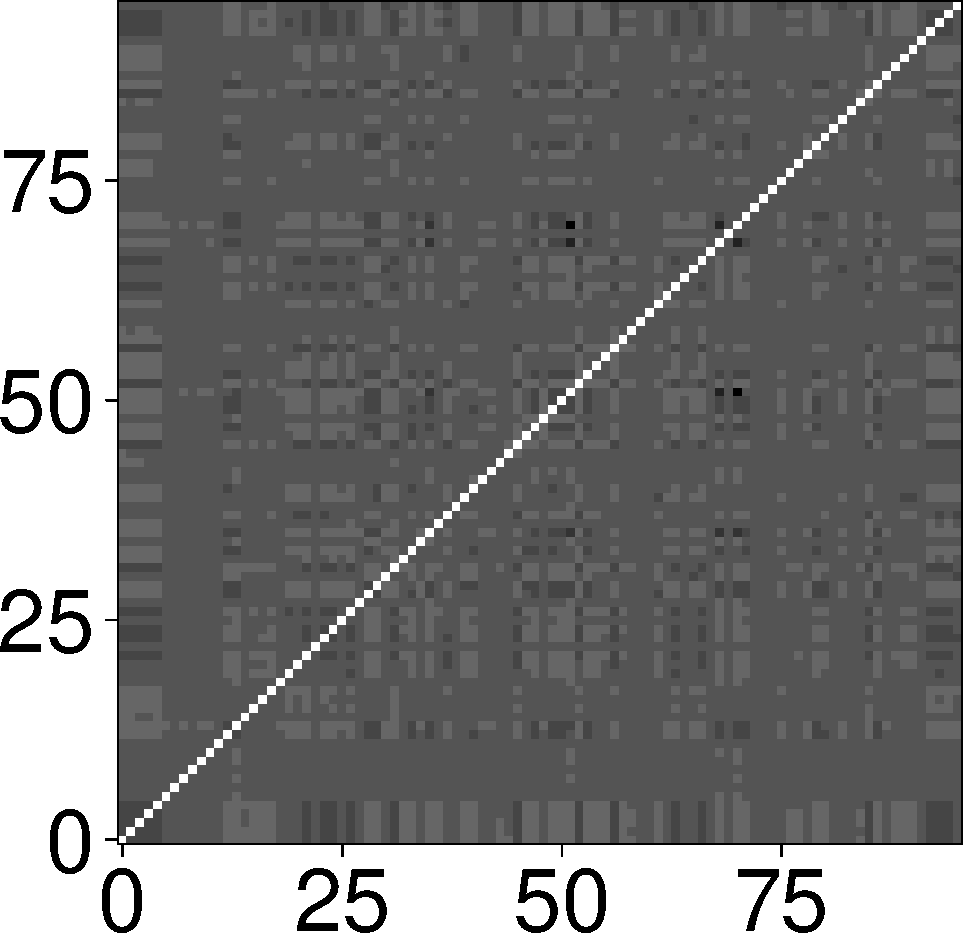
\includegraphics[width=\oneQPage\textwidth]{figures/sharingBehavior/ThirdQ/vacation_96_5.pdf}
		\label{fig:ThirdQvacation962}
	}
	\caption{Matrices with the lowest and highest MSEs.}
	\label{fig:ThirdQMatrices}
\end{figure}
With 96 threads, \emph{vacation} has an all-to-all communication pattern, and the main difference between executions is the total amount of communication, which can be explained by the difference of aborts between each execution. On the other hand, applications such as \emph{genome} present a similar behavior even changing the number of threads, for instance, with 32 threads (\figurename~\ref{fig:ThirdQgenome321} and \figurename~\ref{fig:ThirdQgenome322}).


\subsection{Dynamic behavior during execution}\label{sec:dynamicBehavior}

The goal of this experiment is to determine if the communication pattern changes during the execution of applications. For this experiment, we store multiple communication matrices in different execution phases of the applications. We analyzed the total of addresses accessed by each application (\tablename~\ref{tab:falseSharing}) and used it as a parameter to define a \emph{save interval}, i.e., when to collect the communication matrix. After collection, we reset the data structure responsible to store the communication matrix. For instance, for \emph{labyrinth} the mechanism collected eight matrices, whereas for \emph{kmeans} nineteen matrices were collected.  We run the applications using the default parameters (\tablename~\ref{tab:defaultParams}) and 64 threads.

In the previous sections, the MSE was compared with the first collected matrix, i.e., the baseline was the first execution. For this experiment, the baseline was the last collected matrix. For instance, after two matrices collected it is possible to calculate the MSE between them. When a third matrix is collected, we calculated the MSE between the third and the previous execution (second matrix) onward. \figurename~\ref{fig:dynamicBehavior} presents the results.

\begin{figure}[!t]
	\centering
	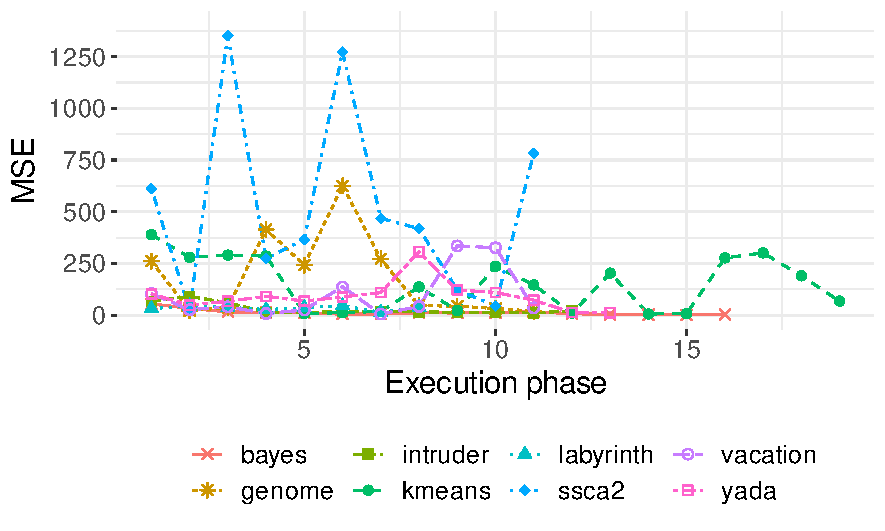
\includegraphics[width=0.9\textwidth]{figures/sharingBehavior/FourthQ/dynamic.pdf}
	\caption{Comparing the MSE on different execution phases.}
	\label{fig:dynamicBehavior}
\end{figure}

Analyzing the graph, \emph{ssca2} has the highest difference in communication patterns during the execution, followed by \emph{genome}. However, as in Sections \ref{sec:sameDIffExecs} and \ref{sec:newInput} the biggest difference in the communication matrices was in the amount of communication between threads since this application has an all-to-all behavior. This is visualized in \figurename~\ref{fig:DynamicMatrices}\subref{fig:Dyssca2-ph1}-\subref{fig:Dyssca2-ph4}.
\begin{figure}[!t]
	\centering
	\subfigure[\emph{ssca2} - phase 1]{
		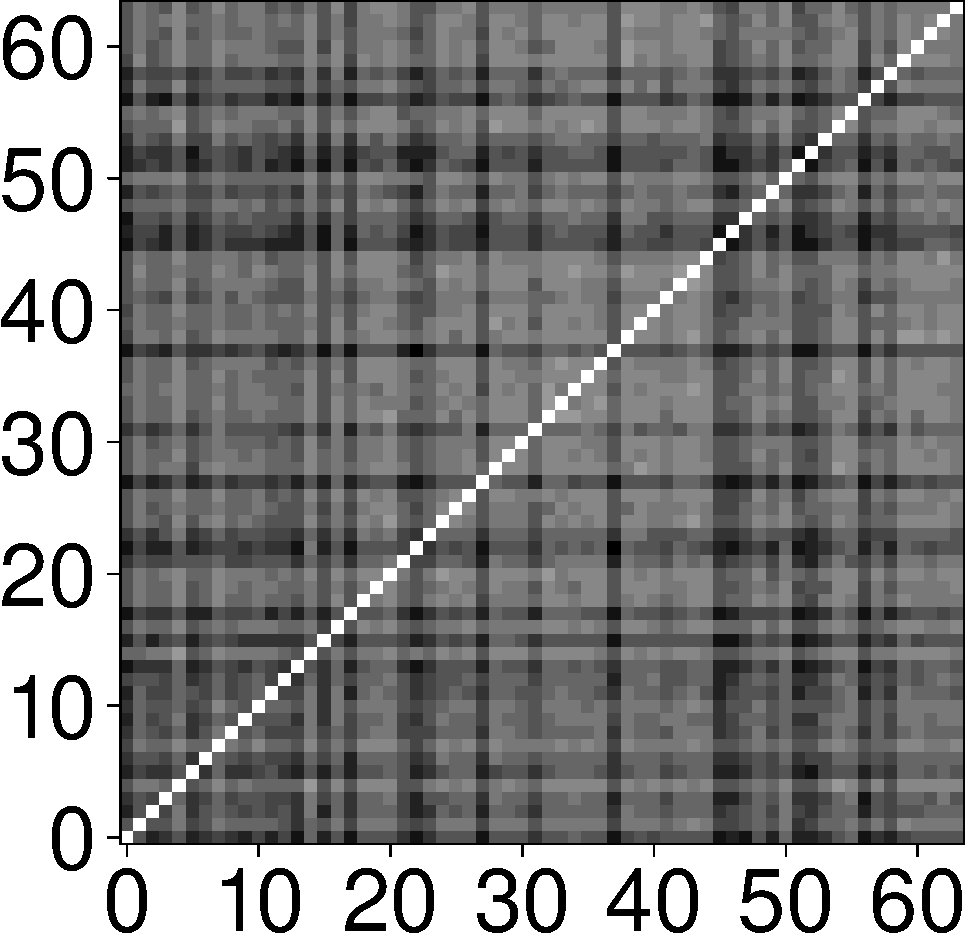
\includegraphics[width=\oneQPage\textwidth]{figures/sharingBehavior/FourthQ/ssca2_64_3.pdf}
		\label{fig:Dyssca2-ph1}
	}
	\subfigure[\emph{ssca2} - phase 2]{
		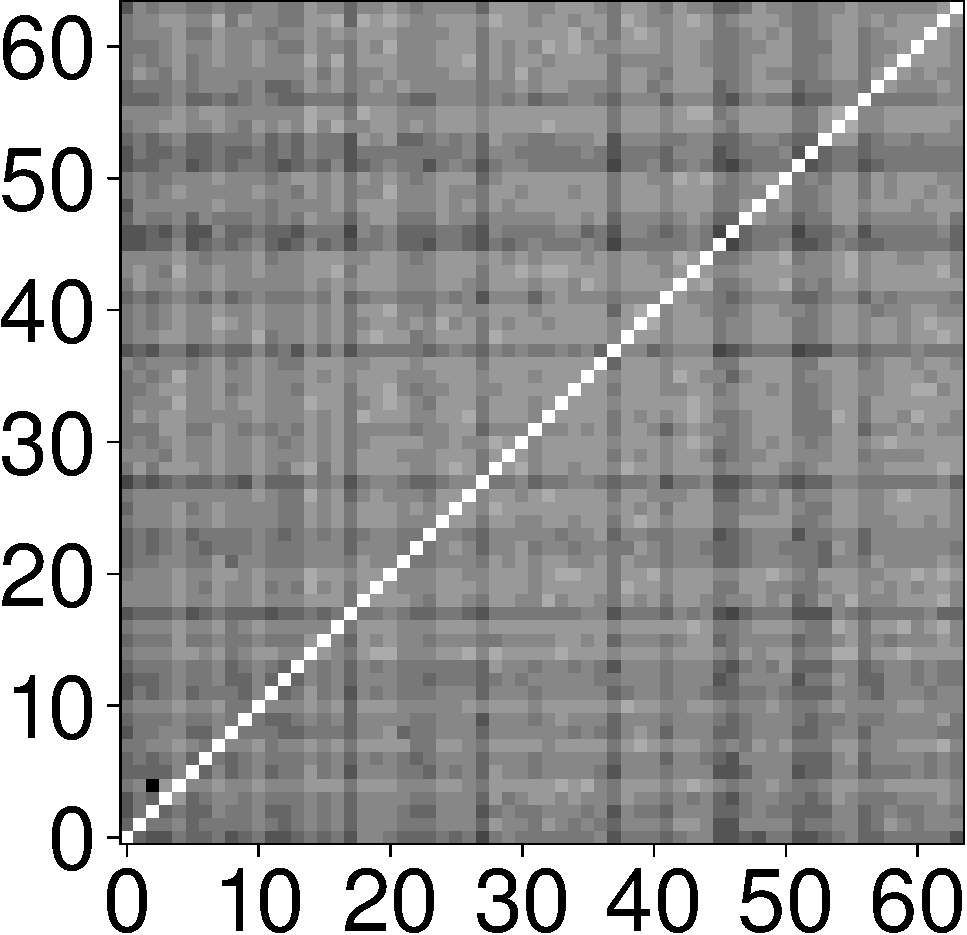
\includegraphics[width=\oneQPage\textwidth]{figures/sharingBehavior/FourthQ/ssca2_64_4.pdf}
	}
	\subfigure[\emph{ssca2} - phase 3]{
		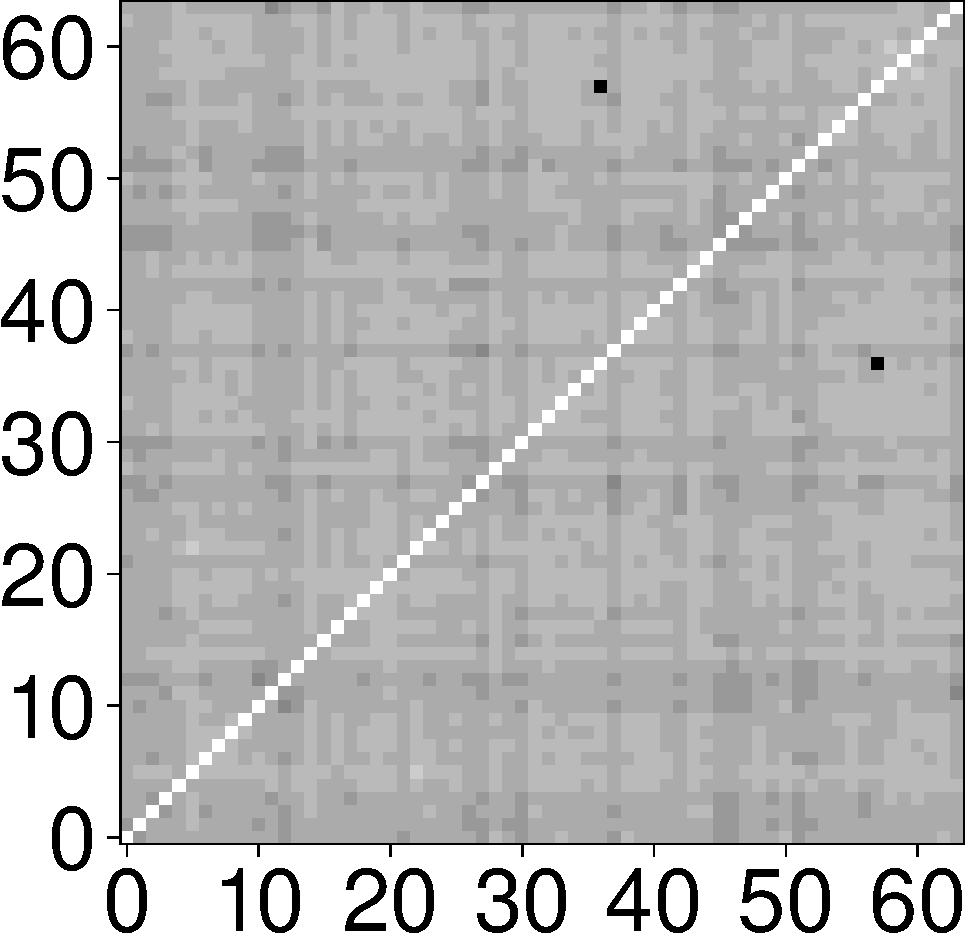
\includegraphics[width=\oneQPage\textwidth]{figures/sharingBehavior/FourthQ/ssca2_64_6.pdf}
	}
	\subfigure[\emph{ssca2} - phase 4]{
		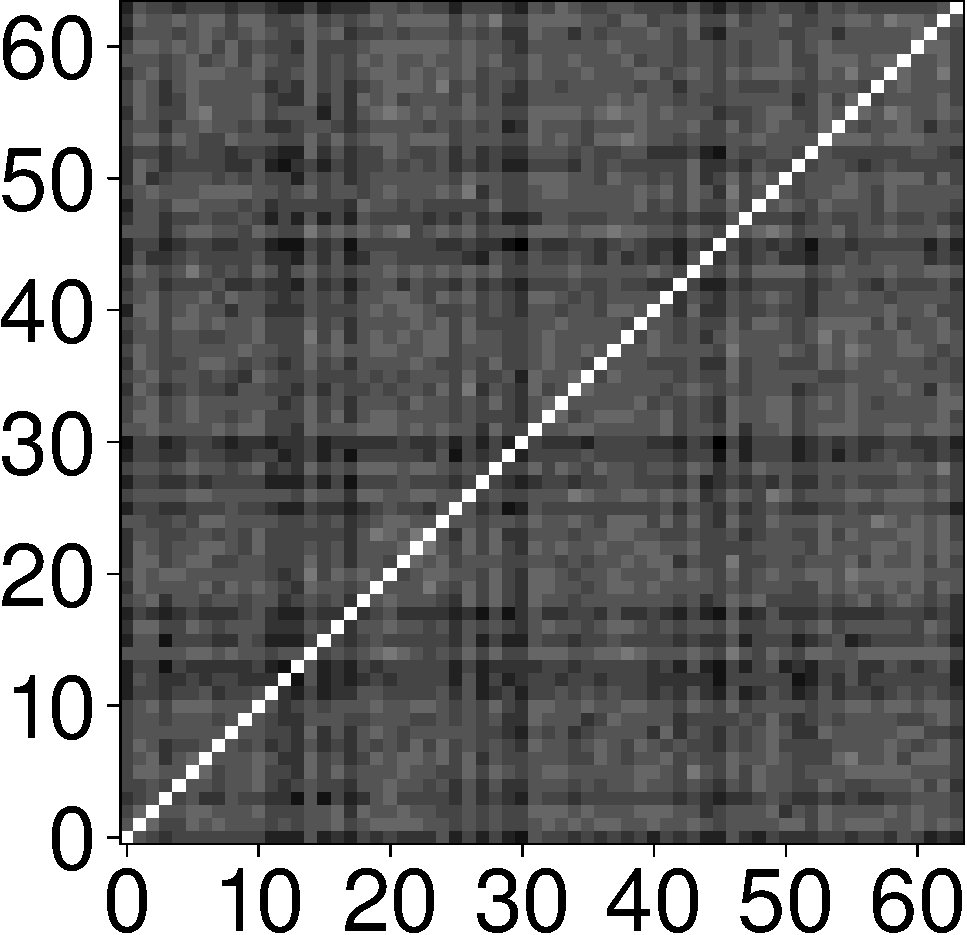
\includegraphics[width=\oneQPage\textwidth]{figures/sharingBehavior/FourthQ/ssca2_64_8.pdf}
		\label{fig:Dyssca2-ph4}
	}
	\\
	\subfigure[\emph{genome} - phase 1]{
		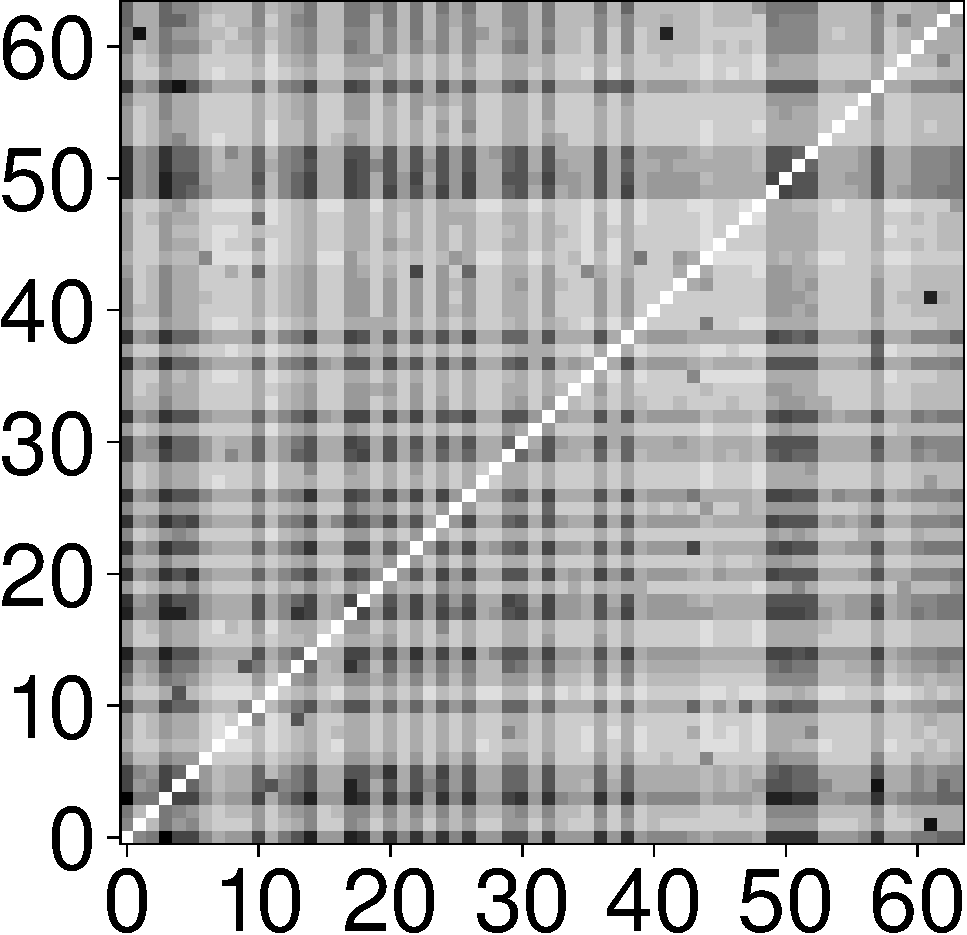
\includegraphics[width=\oneQPage\textwidth]{figures/sharingBehavior/FourthQ/genome_64.pdf}
		\label{fig:Dygenome-ph1}
	}
	\subfigure[\emph{genome} - phase 2]{
		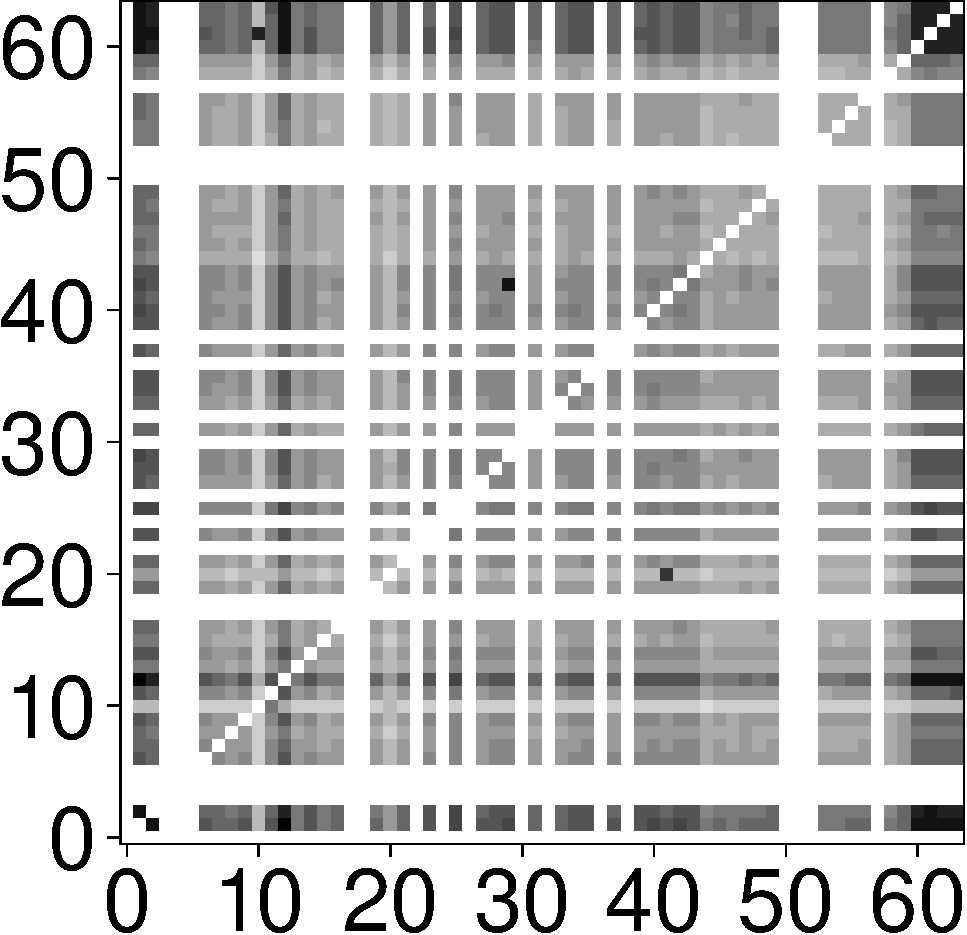
\includegraphics[width=\oneQPage\textwidth]{figures/sharingBehavior/FourthQ/genome_64_5.pdf}
	}
	\subfigure[\emph{genome} - phase 3]{
		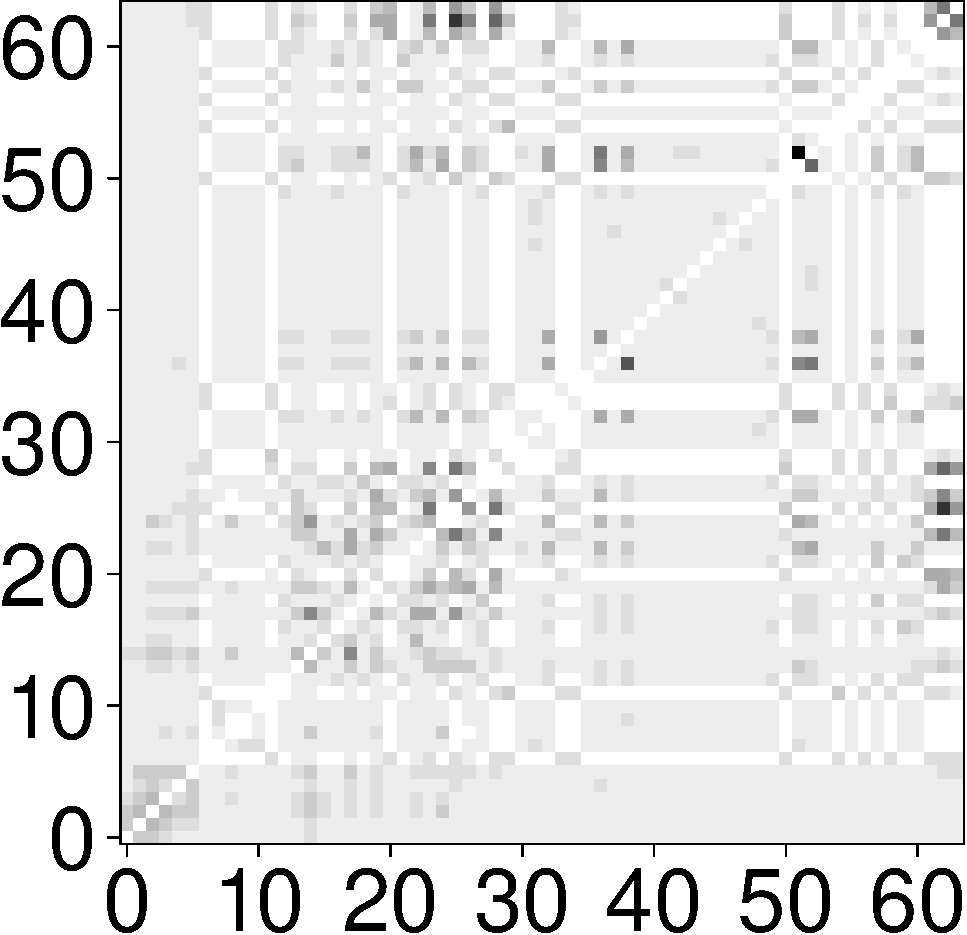
\includegraphics[width=\oneQPage\textwidth]{figures/sharingBehavior/FourthQ/genome_64_9.pdf}
	}
	\subfigure[\emph{genome} -\,phase 4]{
		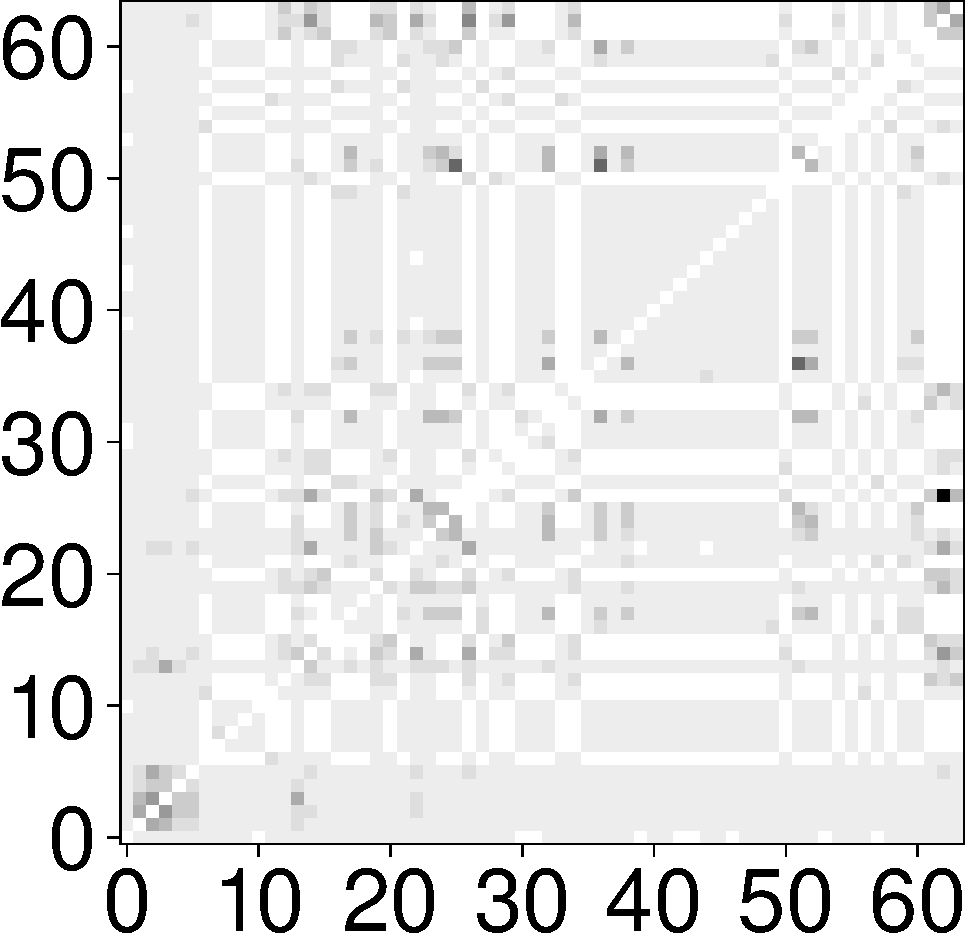
\includegraphics[width=\oneQPage\textwidth]{figures/sharingBehavior/FourthQ/genome_64_11.pdf}
		\label{fig:Dygenome-ph4}
	}
	\caption{Communication matrices in different execution phases.}
	\label{fig:DynamicMatrices}
\end{figure}
On the other hand, \emph{genome} has a varying communication pattern during its execution. There is an intense communication between threads in the beginning of the application, whereas in the end there is little communication (\figurename~\ref{fig:DynamicMatrices}\subref{fig:Dygenome-ph1}-\subref{fig:Dygenome-ph4}). Other applications have a similar communication behavior during their execution.

\section{False sharing in kmeans}


We also performed an experiment to determine if the STM performance can be improved by reducing false sharing (Section~\ref{sec:falseSharing}). %Our modified runtime can provide memory addresses, intensity, and source code locations of false sharing by tracking STM operations that access the same cache lines. 
We selected \texttt{kmeans} for this experiment since it had the highest percentage of false sharing (Table~\ref{tab:falseSharing}). The information collected by our mechanism showed that most of false sharing happened in a matrix of floats (\texttt{new\_centers}) used by \texttt{kmeans}. Analyzing its source code, we identified that the rows of \texttt{new\_centers} were not padded correctly to different cache lines, take into consideration current architectures, 
as showed in the highlighted line (252) in \figurename~\ref{fig:kmeansFalseShare}.
\begin{figure}[!ht]
	\centering
	\fbox{
		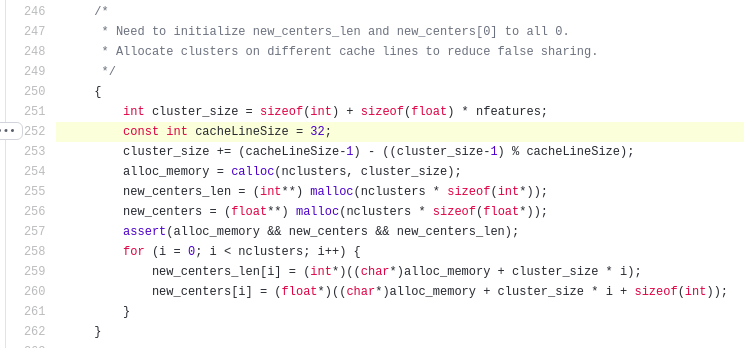
\includegraphics[width=\fullImageWidth\textwidth,trim=15 0 12 0,clip]{figures/sharingBehavior/falseShareKmeans.png}
	}
	\caption{Original source code of kmeans application.}
	\label{fig:kmeansFalseShare}
\end{figure}
The cache line size in current microarchitectures is typically 64 bytes. Probably the developers of the application have used a machine with a cache line size of 32 bytes. Besides, they kept this parameter fixed in the source code. We modified the source code, changing the value of the highlighted line to 64 and obtained performance gains between 4.97\% and 10.97\% compared to the Linux baseline, as shown in Table~\ref{tab:falseSharingKmeans}.


\begin{table}[!t]
	\centering
	\caption{Kmeans performance gains with source code changes to reduce false sharing.}
	\label{tab:falseSharingKmeans}
\begin{tabular}{@{}l@{\hspace*{10pt}}r@{\hspace*{10pt}}r@{\hspace*{10pt}}r@{}}
	\toprule
	& \multicolumn{2}{c}{Execution time} &\\
	\cmidrule(r){2-3}
	\# Threads & Baseline  & Reduced false sharing & Performance gains \\ 
	\midrule
	32                                   & 17.36s                                                                                    & 16.01s                                                                                             & 7.81\%                               \\
	64                                   & 18.05s                                                                                    & 17.15s                                                                                             & 4.97\%                              \\
	96                                   & 19.36s                                                                                     & 17.24s                                                                                             & 10.97\%                              \\ \bottomrule
\end{tabular}
\end{table}

\section{Summary}

This chapter presented a characterization of the \texttt{STAMP} applications regarding their sharing behavior using the mechanism proposed in Chapter~\ref{chap:mechanism}. %We show that by only taking memory accesses from STM operations into consideration, it is possible to create an accurate and low overhead mechanism to determine sharing behavior. 
Since the \texttt{STAMP} benchmark was developed to represent realistic workload characteristics and it covers a wide range of transactional behavior, we expect that the characterization done in this chapter could represent a wide range of real STM applications. The first experiments showed that the sharing behavior of applications does not change between executions using the same configurations, for instance, same input parameters or thread number. Besides, even during execution, the majority of applications do not present a dynamic sharing behavior.
%The major find of the experiments made in this chapter is that the \texttt{STAMP} applications do not present a dynamic sharing behavior during and between executions. 
Hence, our hypothesis is that a \emph{static} thread mapping approach is sufficient to improve the performance of the applications that are suitable for a thread mapping based on their sharing behavior. This hypothesis will be tested in Chapter~(\ref{chap:sharAwareThreadMap}). Beyond that, we were also able to analyze and reduce false sharing in STM memory areas, achieving performance gains when the false sharing was reduced.


%We were also able to analyze and reduce false sharing in STM memory areas, and achieved substantial performance gains from performing thread mapping based on the detected sharing behavior, as well as the reduction of false sharing.